
\paragraph{Task paths}
We can now define the \textit{task-path} as a mapping of atomic tasks to ordered sequence of agents that work together to complete those tasks, $\formalTaskArc{}{}$. In completing an atomic task, the first agent in the sequence is the sink that received the associated composite task. The last agent is the detector that executes the atomic task. The sequence of agents in-between are those agents relaying the atomic task, their position in this sequence denoted by the subscript $i$ where required. So for a task path of depth $n$, we have;
\begin{equation}
	\functionTaskArc{}{} = \lbrace \functionSinkRoleAtomic{}{}, \functionRelayRole{i}{i+1}{}, \functionDetectorRole{}{} \rbrace_{i=2}^{n-1}
\end{equation}
\begin{figure}
	\centering 
	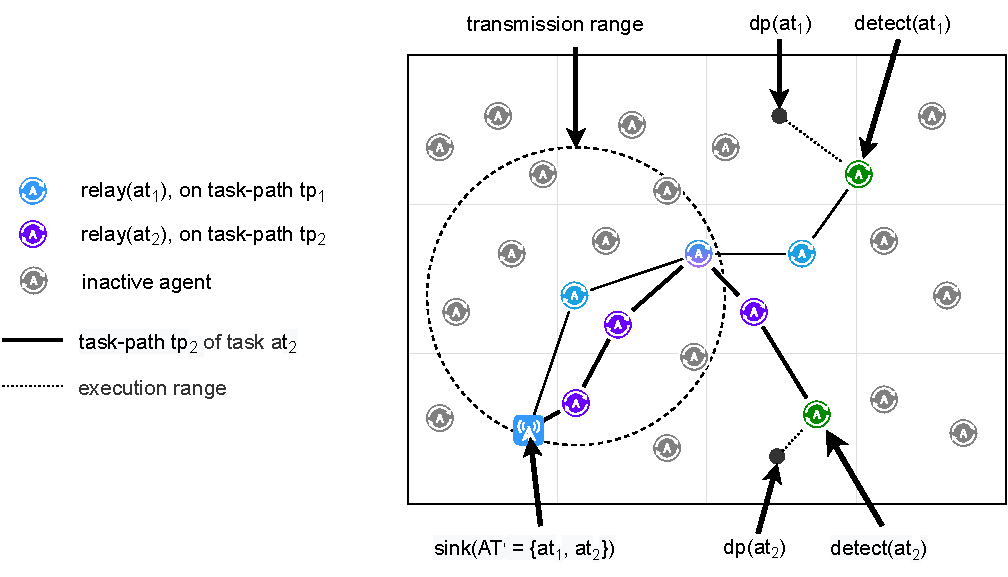
\includegraphics[width=0.9\linewidth, trim={25pt 0pt 24pt 0pt, clip}]{grid_concept}
	\caption[WSN deployment terminology]{WSN components and terminology}
	\label{fig:grid_concept}
\end{figure}
